\documentclass[]{politex}

% ========== Packages ==========
\usepackage[utf8]{inputenc}
\usepackage{amsmath,amsthm,amsfonts,amssymb}
\usepackage{graphicx,cite,enumerate}
\usepackage{subfiles}
\usepackage{caption}
\usepackage{pdfpages}
\usepackage{adjustbox}
\usepackage{wrapfig,lipsum}
\usepackage{verbatim}

% ========== Language options ==========
\usepackage[brazil]{babel}

% ========== ABNT (requer ABNTeX 2) ==========
%	http://www.ctan.org/tex-archive/macros/latex/contrib/abntex2
\usepackage[num]{abntex2cite}

% ========== Lorem ipsum ==========
\usepackage{blindtext}

% ========== Opções do documento ==========
% Título
\titulo{Robô Hospitalar: Hardware e Software}

% Autor
\autor{Vanderson da Silva dos Santos}

% Orientador / Coorientador
\orientador{Leopoldo Rideki Yoshioka}
%\coorientador{Nome do coorientador (opcional)}

% Tipo de documento
\tcc{}
%\dissertacao{Engenharia Elétrica}
%\teseDOC{Engenharia Elétrica}
%\teseLD
%\memorialLD

% Departamento e área de concentração
\departamento{Engenharia de Sistemas Eletrônicos}
\areaConcentracao{Engenharia de Sistemas Eletrônicos}

% Local
\local{São Paulo}

% Ano
\data{2021}

\begin{document}
% ========== Capa e folhas de rosto ==========
\capa
\falsafolhaderosto
\folhaderosto

%========== Folha de assinaturas (opcional) ==========
%\begin{folhadeaprovacao}
	\assinatura{Prof. Dr. Leopoldo Rideki Yoshioka}
%	\assinatura{Prof.\ Y}
%	\assinatura{Prof.\ Z}
%\end{folhadeaprovacao}

% ========== Ficha catalográfica ==========
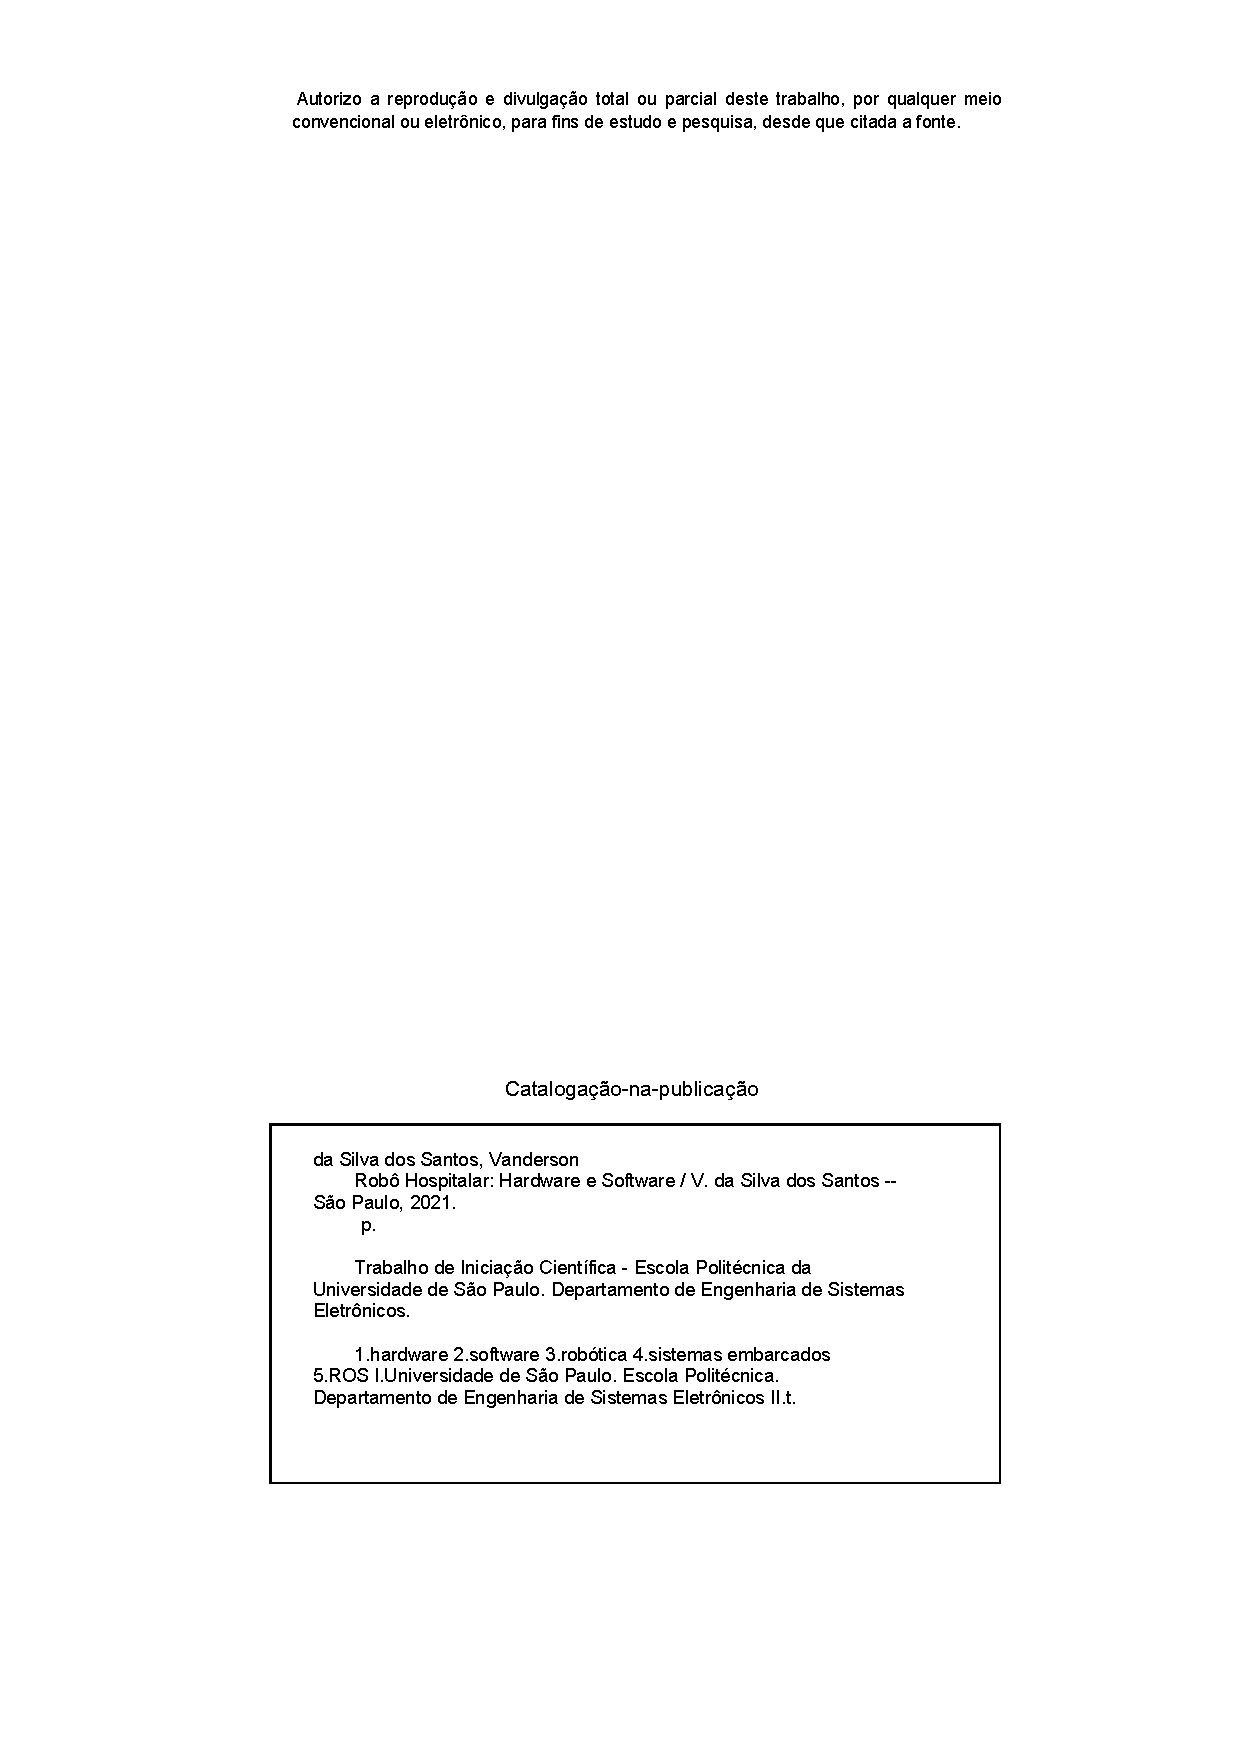
\includepdf{ficha_catalografica.pdf}

% ========== Dedicatória (opcional) ==========
\dedicatoria{Dedico esse trabalho aos amigos do Robô Hospitalar}

% ========== Agradecimentos ==========
\begin{agradecimentos}

Thanks...

\end{agradecimentos}

% ========== Epígrafe (opcional) ==========
\epigrafe{%
	\emph{``Mas nunca imaginaria que a curiosidade fosse outra dessas tantas ciladas do amor''}
	\begin{flushright}
		- Gabriel Garcia Marquez
	\end{flushright}
}

% ========== Resumo ==========
\begin{resumo}
Resumo...
%
\\[3\baselineskip]
%
\textbf{Palavras-Chave} -- Palavra, Palavra, Palavra, Palavra, Palavra.
\end{resumo}

% ========== Abstract ==========
\begin{abstract}
Abstract...
%
\\[3\baselineskip]
%
\textbf{Keywords} -- Word, Word, Word, Word, Word.
\end{abstract}

% ========== Listas (opcional) ==========
\listadefiguras
\listadetabelas

% ========== Sumário ==========
\sumario

% ========== Elementos textuais ==========

% ========== Parte 1: Introdução ==========
\part{Introdução}
\subfile{chapters/introducao}

\subfile{chapters/objetivo}

\subfile{chapters/motivacao}

\subfile{chapters/metodologia}

\subfile{chapters/arquitetura_do_projeto}

% ========== Parte 2: Hardware ==========
\part{Hardware}

\subfile{chapters/modulos_embarcados}

\subfile{chapters/distribuicao_de_energia}
% ========== Parte 3: Software ==========
\part{Software}

\subfile{chapters/sistema_computacional_completo}

\subfile{chapters/ambiente_de_simulacao}

\subfile{chapters/algoritmos_de_controle}

\blindtext

\begin{citacaoLonga}
	\blindtext
\end{citacaoLonga}

\blindtext

% ========== TITULOS DO SUMÁRIOS ==========
%\blinddocument
% =========================================

% ========== Referências ==========
% --- ABNT (requer ABNTeX 2) ---
%	http://www.ctan.org/tex-archive/macros/latex/contrib/abntex2
\bibliographystyle{abntex2-num}
\bibliography{bibliography}

% ========== Apêndices (opcional) ==========
\apendice
\chapter{}
\chapter{Beta}

% ========== Anexos (opcional) ==========
\anexo
\chapter{Alpha}
\chapter{}

\end{document}